\documentclass{beamer}
\usepackage[utf8]{inputenc}
\usepackage{xmpmulti}
%\usetheme{JuanLesPins}
\usetheme{Padova}

%STRUTTURA:
%DTN
%M2MShare
%ONE
%modelli movimento: WDM

          
\author{Daniele Bonaldo}
\title{Performance Evaluation with Realistic Mobility of a File Sharing DTN Protocol}
\institute{UNIVERSITA' DEGLI STUDI DI PADOVA\\
Facoltà di Scienze MM. FF. NN.\\
Corso di Laurea Magistrale in Informatica
}
\date{23 settembre 2011}

\begin{document}

\maketitle
%\begin{frame}[t,plain]
%\titlepage
%\end{frame}

%\begin{frame}[t,fragile]
%\frametitle{Sommario}
%\begin{enumerate}
%\item DTN e M2MShare
%\item Obiettivi del progetto
%\item The ONE simulator
%\item Modelli di movimento
%\item Descrizione delle simulazioni
%\item Risultati
%\end{enumerate}
%\end{frame}

\begin{frame}
\frametitle{Obiettivi del progetto}
\begin{itemize}
\item Implementare M2MShare in un ambiente di simulazione che permetta di valutarne l'efficienza considerando la mobilità dei nodi interessati
\item Confrontare l'efficienza di M2MShare rispetto altre strategie applicabili nello stesso contesto
\item Migliorare la versione esistente del protocollo 
\end{itemize}
\end{frame}

%\begin{frame}[t,fragile]
%\frametitle{DTN - Delay Tolerant Networks}
%\ \\
%Caratterizzate da interruzioni frequenti di connettività\\
%Difficoltà di instaurare un link sorgente-destinazione permanente\\
%Ne segue inefficienza dei protocolli di routing tradizionali\\
%\end{frame}

\begin{frame}
\frametitle{DTN - Delay Tolerant Networks}

Caratterizzate da interruzioni frequenti di connettività\\
Difficoltà di instaurare un link sorgente-destinazione permanente\\
Ne segue inefficienza dei protocolli di routing tradizionali\\
\ \\
\pause 
Una soluzione:\\
\ \\
\begin{center}
\textbf{Store-carry-forward}\\
\end{center}

Non si mantiene un collegamento continuo fra la sorgente e la destinazione ma i nodi intermedi trasportano i pacchetti dalla sorgente alla destinazione muovendosi.
\end{frame}




\begin{frame}
\frametitle{M2MShare}
%\textbf{Problema: } un nodo in una DTN può non coprire abbastanza spazio durante i propri movimenti per raggiungere il destinatario dei dati che sta trasportando.
%\ \\
%\ \\
%\pause 
\textbf{M2MShare} aggiunge il sistema delle deleghe e lo utilizza all'interno di un protocollo Peer-to-peer per lo scambio di files fra dispositivi mobili.
\ \\
\ \\
\pause 
Dispositivi dotati di:
\begin{itemize}
\item elevata mobilità
\item limitata autonomia energetica
\item limitato raggio di comunicazione
\item limitato spazio di storage
\end{itemize}
\end{frame}

\begin{frame}
\frametitle{M2MShare}
Mentre l'elevata mobilità dei dispositivi costituirebbe un problema per dei protocolli tradizionali, M2MShare utilizza tale mobilità, assieme al sistema delle deleghe per ampliare l'area esplorata dai nodi interessati nella ricerca di un file.
\end{frame}

\begin{frame}
\frametitle{The ONE simulator}
Simulatore che permette di emulare il comportamento dei nodi all'interno della rete in un  ambiente realistico, utilizzando diversi modelli di movimento di diversa complessità.
\end{frame}

\begin{frame}
\frametitle{Movement Models}
ONE contiene al suo interno diversi Movement Models:
\begin{itemize}
\item Random Walk Movement
\item Random Waypoint Movement
\pause
\item Random Map-Based Movement
\item Shortest Path Map-Based Movement
\item Routed Map-Based Movement
\end{itemize}
\ \\
\pause
Più adatto alle nostre simulazioni:
\begin{center}
\textbf{Working Day Movement Model}
\end{center}
\end{frame}

\begin{frame}
\frametitle{Movement Models - WDM}
\textbf{Working Day Movement Model} (WDM)\\
simula la ripetitività delle azioni giornaliere svolte dalle persone durante i giorni lavorativi:
\begin{itemize}
\item Dormire a casa
\item Andare a lavoro in ufficio
\item Uscire dopo il lavoro per shopping / serata con gli amici
\end{itemize}
\ \\
\pause
Utilizza diversi sottomodelli per simulare diverse possibilità per i nodi di muoversi all'interno della mappa:
\begin{itemize}
\item camminando
\item guidando un mezzo proprio
\item utlizzare mezzi pubblici che si muovono secondo rotte prefissate
\end{itemize}
\end{frame}

\begin{frame}
\frametitle{La Mappa}
Mappa del centro cittadino di Helsinki:
\begin{figure}[htpb]

\begin{minipage}[b]{0.5\linewidth}
  \begin{center}
  	\multiinclude[format=png,graphics={scale=0.18}]{../figure/mappa/mappa}
%    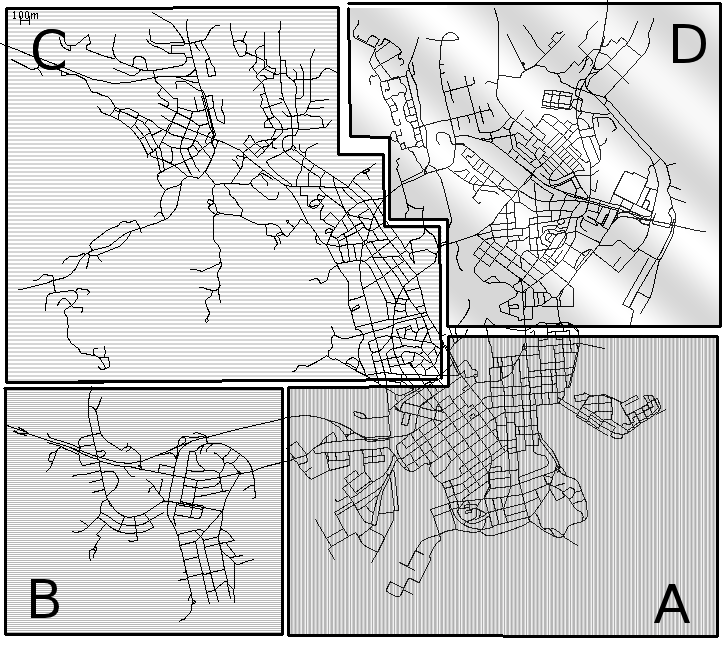
\includegraphics[scale=0.18]{../figure/mappa_ABCD.png}      
    \label{imgMappaABCD}
  \end{center}
\end{minipage}

\hspace{0.5cm}


\begin{minipage}[b]{0.5\linewidth}
\tiny 

\begin{center}
\begin{tabular}{|l|c|c|c|}
\hline
\textbf{District} & \textbf{Nodes} & \textbf{Offices} & \textbf{Meeting spots}\\
\hline
\hline
\bfseries A & 150 & 30 & 4 \\
\hline
\bfseries B & 50 & 10 & 1 \\
\hline
\bfseries C & 100 & 20 & 2 \\
\hline
\bfseries D & 100 & 20 & 2 \\
\hline
\bfseries E (A + B) & 100 & 20 & 2 \\
\hline
\bfseries F (A + C) & 150 & 30 & 4 \\
\hline
\bfseries G (A + D) & 150 & 30 & 4 \\
\hline
\bfseries H (Whole map) & 200 & 40 & 5 \\
\hline
\end{tabular}
\end{center}   
\label{tabellaDistrettiMappa}

\normalsize
\end{minipage}

\end{figure}
\end{frame}
%
%\begin{frame}
%\frametitle{Simulazioni}
%Obiettivo: analizzare l'efficienza di M2MShare in termini di tempo di recupero del file cercato rispetto ad altre due strategie, una che non utilizza deleghe, l'altra in cui si delegano task indiscriminatamente a tutti i nodi incontrati.
%\small
%\begin{table}[h]
%\begin{center}
%\begin{tabular}{|l|r|}
%\hline
%\bfseries Population & 1000 \\
%\hline
%\bfseries File size & 3.0 MB \\
%\hline
%\bfseries File popularity & 50 copies uniformly chosen \\
%\hline
%\bfseries Delegation type & No\_delegation, M2MShare, Delegation\_to\_all \\
%\hline
%\bfseries Delegation depth & 1 \\
%\hline
%\bfseries File Division Strategy & M2MShare \\
%\hline
%\bfseries Nr. of simulations & 40 x 3\\
%\hline
%\bfseries Simulated time & One week \\
%\hline
%\end{tabular}
%\end{center}
%\end{table}
%\normalsize
%\end{frame}
%
%\begin{frame}
%\frametitle{Simulazioni}
%Obiettivo: analizzare l'efficienza di M2MShare rispetto alle altre due strategie, con diversi valori di popolarità del file cercato.
%\small
%\begin{table}[h]
%\begin{center}
%\begin{tabular}{|l|r|}
%\hline
%\bfseries Population & 1000 \\
%\hline
%\bfseries File size & 3.0 MB \\
%\hline
%\bfseries File popularity & 50, 100, 150, 200, 250, 300, 350, 400 copies \\
%\hline
%\bfseries Delegation type & No\_delegation, M2MShare, Delegation\_to\_all \\
%\hline
%\bfseries Delegation depth & 1 \\
%\hline
%\bfseries File Division Strategy & M2MShare \\
%\hline
%\bfseries Nr. of simulations & 40 x 8 x 3\\
%\hline
%\bfseries Simulated time & 48 hours \\
%\hline
%\end{tabular}
%\end{center}
%\end{table}
%\normalsize
%\end{frame}
%
%\begin{frame}
%\frametitle{Simulazioni}
%Obiettivo: analizzare l'efficienza di M2MShare rispetto alle altre due strategie, con diversi valori di popolazione totale nel mondo simulato.
%\small
%\begin{table}[h]
%\begin{center}
%\begin{tabular}{|l|r|}
%\hline
%\bfseries Population & 100, 200, 400, 600, 800, 1000 \\
%\hline
%\bfseries File size & 3.0 MB \\
%\hline
%\bfseries File popularity & 5\%, 10\%, 50\% \\
%\hline
%\bfseries Delegation type & No\_delegation, M2MShare, Delegation\_to\_all \\
%\hline
%\bfseries Delegation depth & 1 \\
%\hline
%\bfseries File Division Strategy & M2MShare \\
%\hline
%\bfseries Nr. of simulations & 40 x 6 x 3 x 3\\
%\hline
%\bfseries Simulated time & 48 hours \\
%\hline
%\end{tabular}
%\end{center}
%\end{table}
%\normalsize
%\end{frame}
%
%\begin{frame}
%\frametitle{Simulazioni}
%Obiettivo: analizzare l'efficienza di M2MShare originale (1-hop delegations) rispetto alla nostra versione aggiornata (con deleghe fino a 3 hop)
%\small
%\begin{table}[h]
%\begin{center}
%\begin{tabular}{|l|r|}
%\hline
%\bfseries Population & 1000 \\
%\hline
%\bfseries File size & 3.0 MB \\
%\hline
%\bfseries File popularity & 25 copies in a single district \\
%\hline
%\bfseries Delegation type & No\_Delegation, M2MShare\\
%\hline
%\bfseries Delegation depth & 1, 3 \\
%\hline
%\bfseries File Division Strategy & M2MShare \\
%\hline
%\bfseries Nr. of simulations & 40 x 3\\
%\hline
%\bfseries Simulated time & One week \\
%\hline
%\end{tabular}
%\end{center}
%\end{table}
%\normalsize
%\end{frame}
%
%\begin{frame}
%\frametitle{Simulazioni}
%Obiettivo: analizzare l'efficienza di M2MShare in termini di ridondanza totale di dati generata all'interno della rete.
%\small
%\begin{table}[h]
%\begin{center}
%\begin{tabular}{|l|r|}
%\hline
%\bfseries Population & 1000 \\
%\hline
%\bfseries File size & 3.0 MB \\
%\hline
%\bfseries File popularity & 50 copies uniformly chosen \\
%\hline
%\bfseries Delegation type & M2MShare, Delegation\_to\_all \\
%\hline
%\bfseries Delegation depth & 1 \\
%\hline
%\bfseries File Division Strategy & M2MShare \\
%\hline
%\bfseries Nr. of simulations & 40 x 2\\
%\hline
%\bfseries Simulated time & One week \\
%\hline
%\end{tabular}
%\end{center}
%\end{table}
%\normalsize
%\end{frame}
%
%\begin{frame}
%\frametitle{Simulazioni}
%Obiettivo: analizzare l'efficienza della File Division Strategy di M2MShare rispetto ad altre due tecniche, una in cui ogni trasferimento di file comincia dall'inizio del file, l'altra in cui il punto iniziale del trasferimento viene scelto casualmente per ogni trasferimento.
%\small
%\begin{table}[h]
%\begin{center}
%\begin{tabular}{|l|r|}
%\hline
%\bfseries Population & 1000 \\
%\hline
%\bfseries File size & 3.0 MB, 10.0 MB, 25.0 MB \\
%\hline
%\bfseries File popularity & 50 copies uniformly chosen \\
%\hline
%\bfseries Delegation type & M2MShare \\
%\hline
%\bfseries Delegation depth & 1 \\
%\hline
%\bfseries File Division Strategy & M2MShare, iM , rM \\
%\hline
%\bfseries Nr. of simulations & 40 x 3 x 3\\
%\hline
%\bfseries Simulated time & One week \\
%\hline
%\end{tabular}
%\end{center}
%\end{table}
%\normalsize
%\end{frame}

\begin{frame}
\frametitle{Risultati}
\textbf{Obiettivo:} analizzare l'efficienza di M2MShare in termini di tempo di recupero del file cercato rispetto ad altre due strategie, una che non utilizza deleghe, l'altra in cui si delegano task indiscriminatamente a tutti i nodi incontrati.
\end{frame}

\begin{frame}
\frametitle{Risultati}
\begin{center}
\begin{figure}[ht]
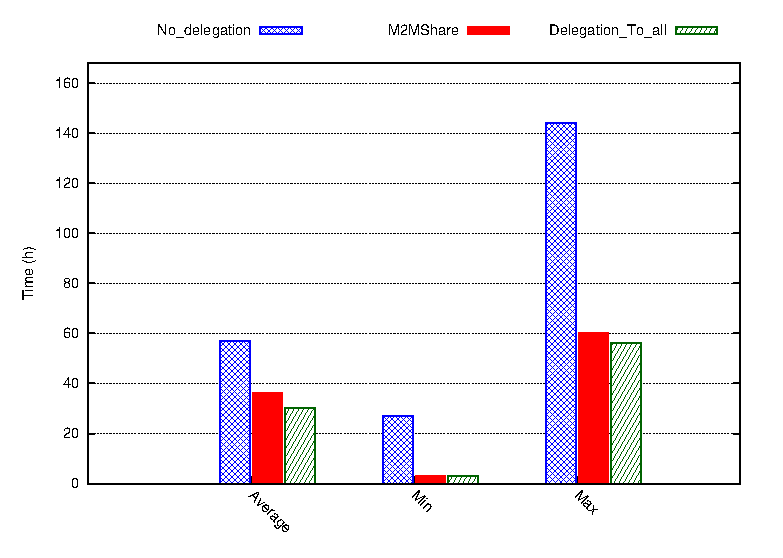
\includegraphics[scale=0.7]{../grafici/tempi.eps}
\caption{Average, min. max found time employed by each strategy in finding the required data file.}
\end{figure}
\end{center}
\end{frame}

\begin{frame}
\frametitle{Risultati}
\begin{figure}[ht]
\begin{minipage}[b]{0.45\linewidth}
\centering
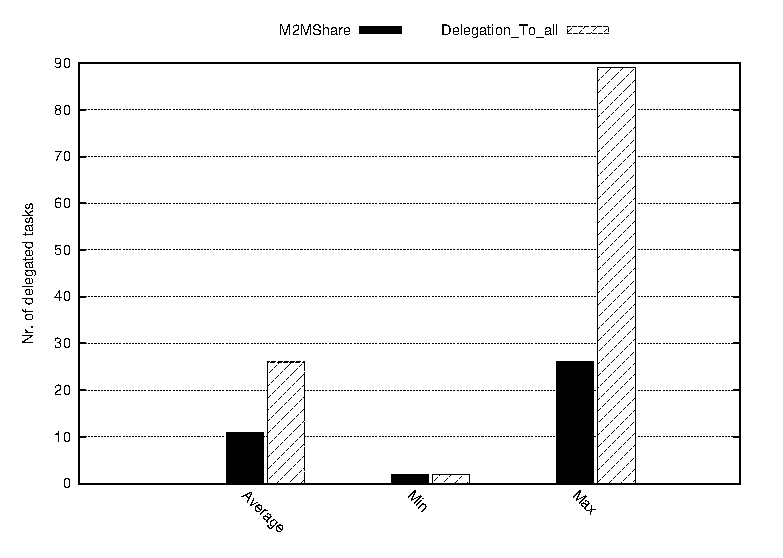
\includegraphics[scale=0.4]{../grafici/delegheFatte.eps}
\caption{Average, min, max number of delegations employed by each delegation strategy.}
\end{minipage}
\hspace{0.5cm}
\begin{minipage}[b]{0.45\linewidth}
\centering
\pause
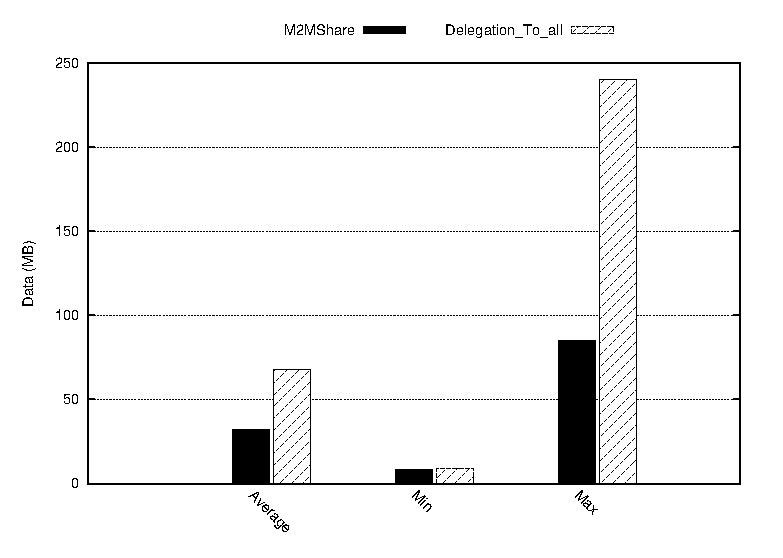
\includegraphics[scale=0.4]{../grafici/data.eps}
\caption{Average, min, max number of delegations employed by each delegation strategy.}
\end{minipage}
\end{figure}
\end{frame}


\begin{frame}
\frametitle{Risultati}
\begin{figure}[ht]
\begin{minipage}[b]{0.4\linewidth}
\centering
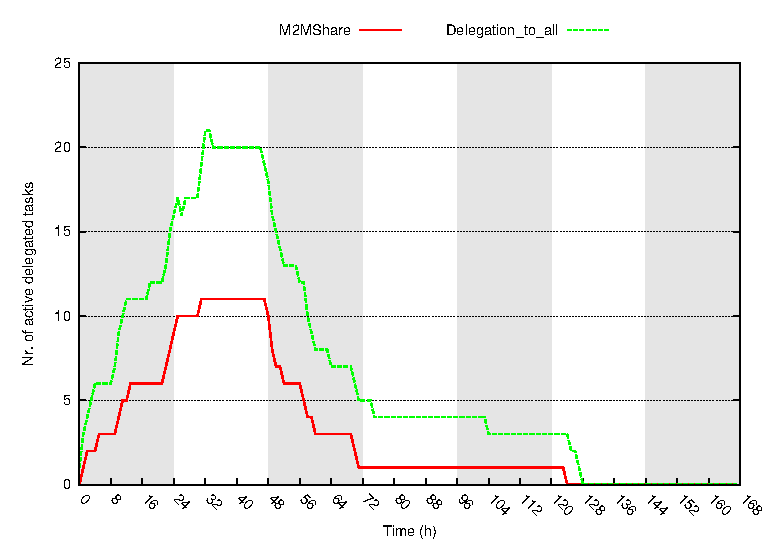
\includegraphics[scale=0.4]{../grafici/delegheAttive.eps}
%\caption{Average number of simultaneously active delegated tasks}
\end{minipage}

%\hspace{0.5cm}

%\begin{minipage}[b]{0.40\linewidth}
%\centering
%\pause
%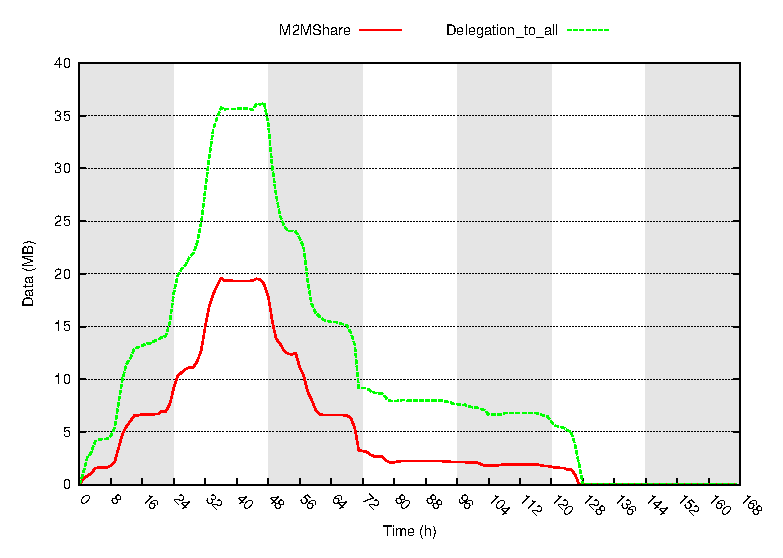
\includegraphics[scale=0.3]{../grafici/ridondanza.eps}
%\caption{Average data redundancy in the network}
%\end{minipage}

\begin{minipage}[b]{0.4\linewidth}
\centering
\pause
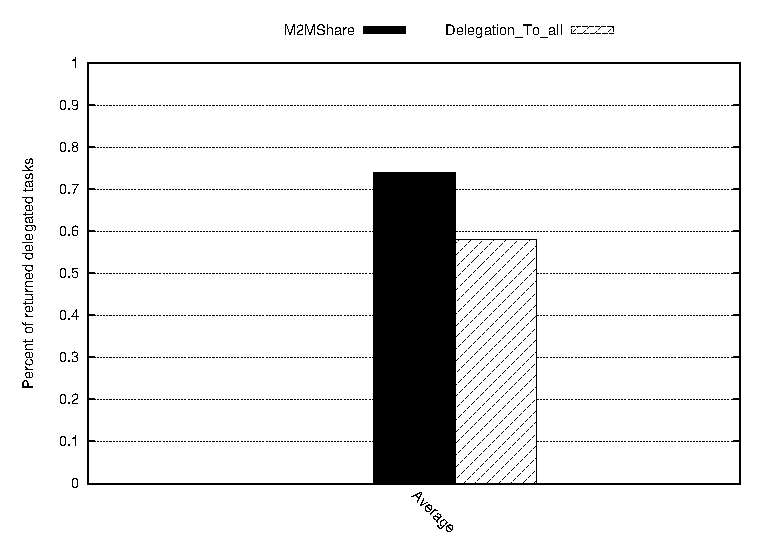
\includegraphics[scale=0.4]{../grafici/percDeleghe.eps}
%\caption{Percentage of completed previously delegated tasks against the number of overall delegations employed.}
\end{minipage}

\end{figure}
\end{frame}


\begin{frame}
\frametitle{Risultati}
\begin{center}
\begin{figure}[ht]
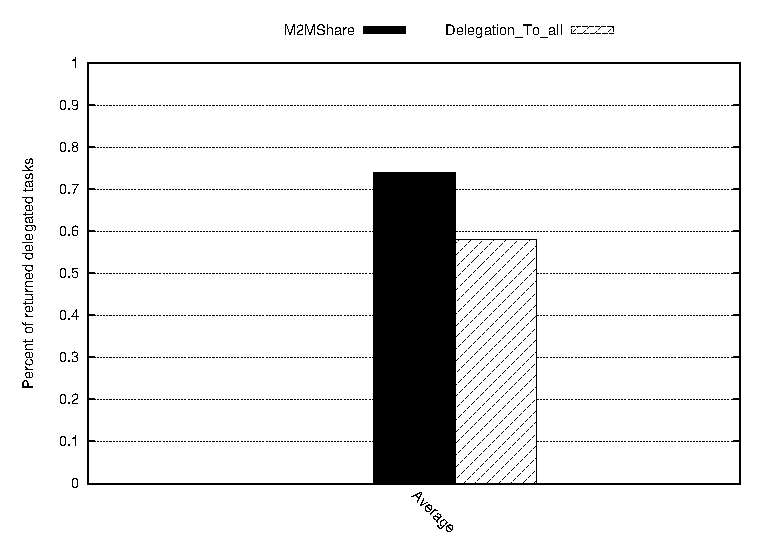
\includegraphics[scale=0.7]{../grafici/percDeleghe.eps}
\caption{Percentage of completed previously delegated tasks against the number of overall delegations employed.}
\end{figure}
\end{center}
\end{frame}

\begin{frame}
\frametitle{Risultati}
\begin{center}
\begin{figure}[ht]
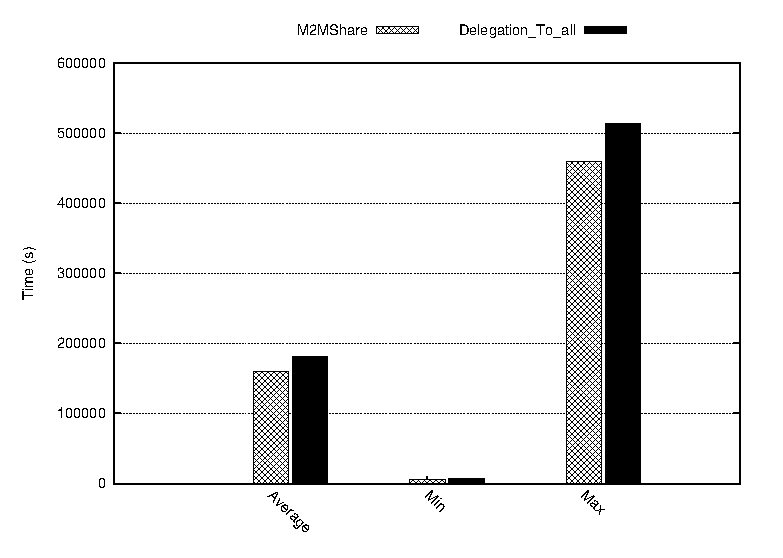
\includegraphics[scale=0.7]{../grafici/tempiRitornoDeleghe.eps}
\caption{Average, min, max output return time for systems using task delegations.}
\end{figure}
\end{center}
\end{frame}

\begin{frame}
\frametitle{Risultati}
\begin{center}
\begin{figure}[ht]
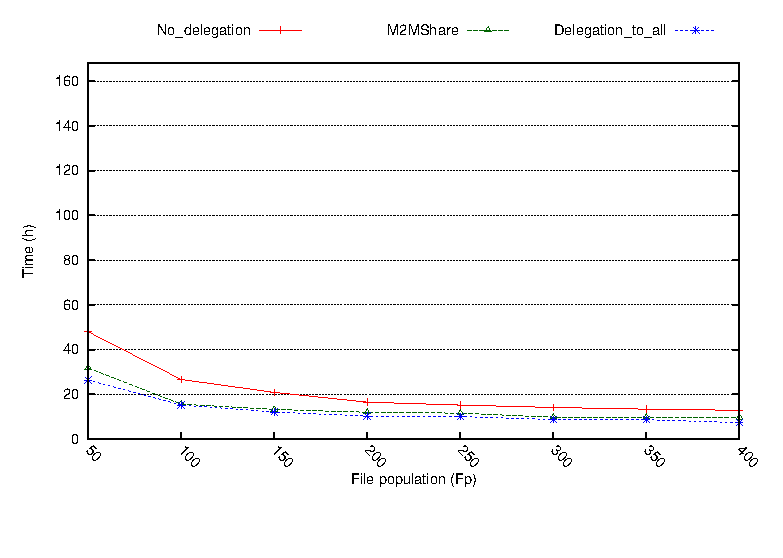
\includegraphics[scale=0.7]{../grafici/tempiVFDiversaPop.eps}
    \caption{Percentage of completed previously delegated tasks against the number of overall delegations employed.}
\end{figure}
\end{center}
\end{frame}

\begin{frame}
\frametitle{Risultati}
\begin{center}
\begin{figure}[ht]
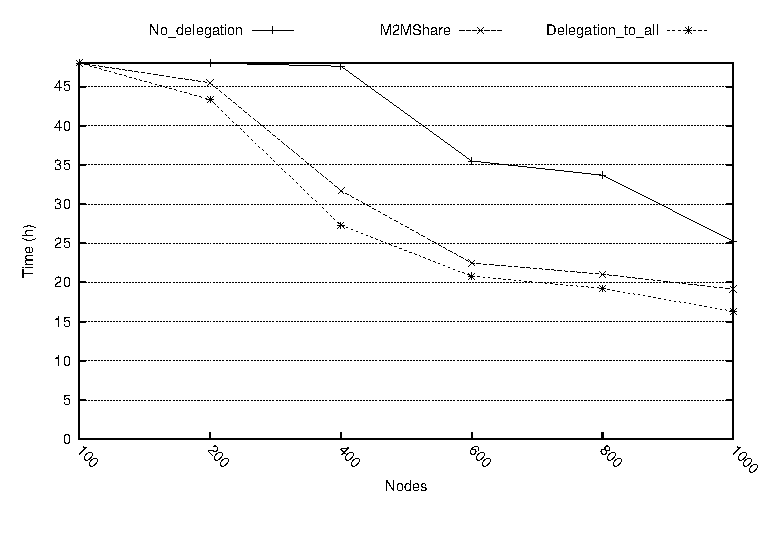
\includegraphics[scale=0.7]{../grafici/tempiVF_Fp5.eps}
\caption{Average found time with $Fp = 5\%$}
\end{figure}
\end{center}
\end{frame}

\begin{frame}
\frametitle{Risultati}
\begin{center}
\begin{figure}[ht]
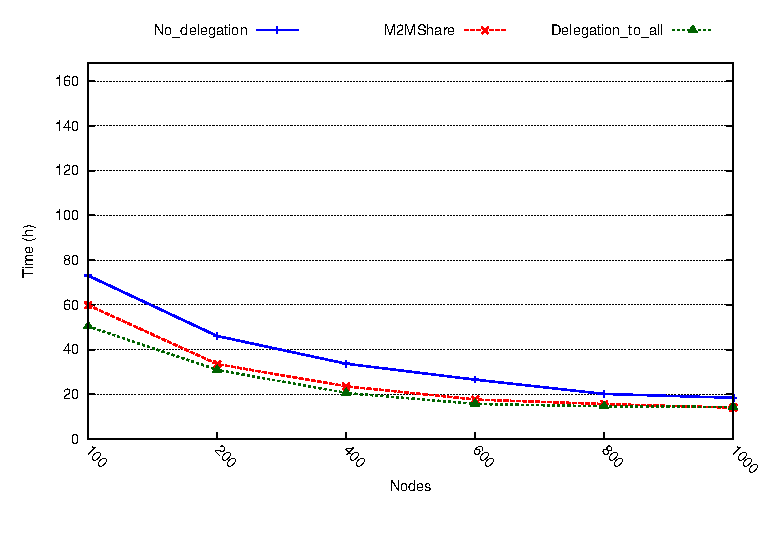
\includegraphics[scale=0.7]{../grafici/tempiVF_Fp10.eps}
\caption{Average found time with $Fp = 10\%$}
\end{figure}
\end{center}
\end{frame}

\begin{frame}
\frametitle{Risultati}
\begin{center}
\begin{figure}[ht]
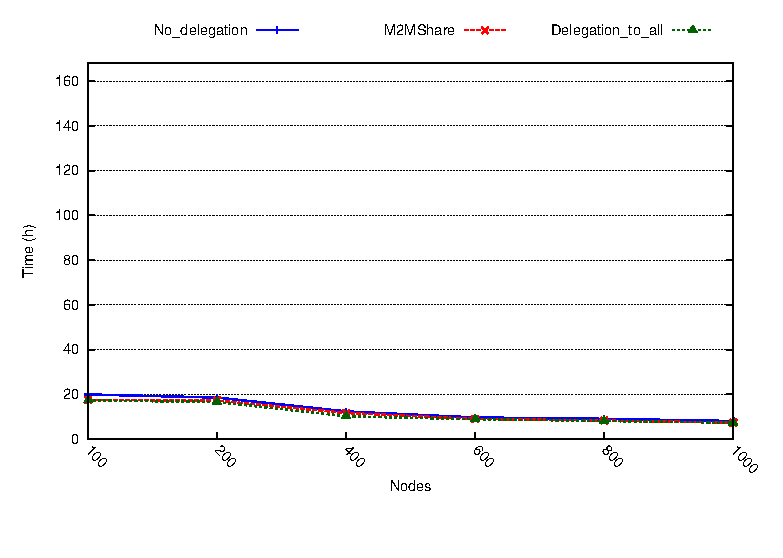
\includegraphics[scale=0.7]{../grafici/tempiVF_Fp50.eps}
\caption{Average found time with $Fp = 50\%$}
\end{figure}
\end{center}
\end{frame}

\begin{frame}
\frametitle{Risultati}
\begin{center}
\begin{figure}[ht]
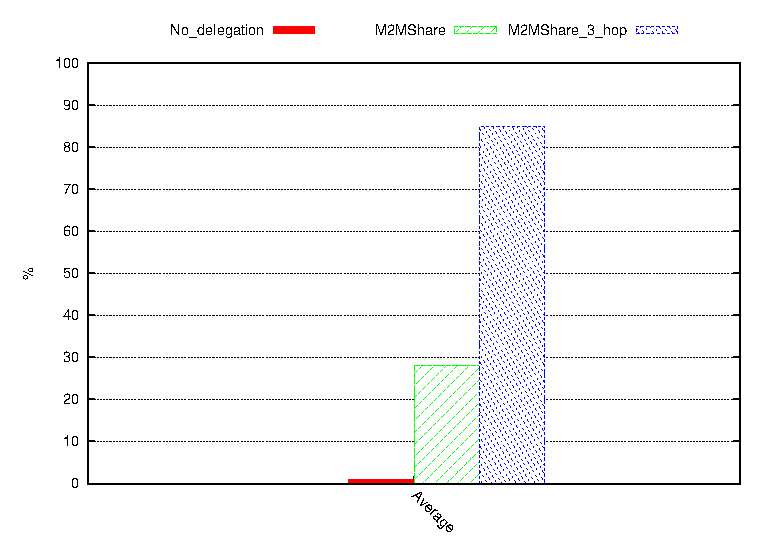
\includegraphics[scale=0.7]{../grafici/percCompletaMultiHop.eps}
\caption{Percentage of successfully completed simulations with searched file far from requester.}
\end{figure}
\end{center}
\end{frame}

\begin{frame}
\frametitle{Risultati}
\begin{center}
\begin{figure}[ht]
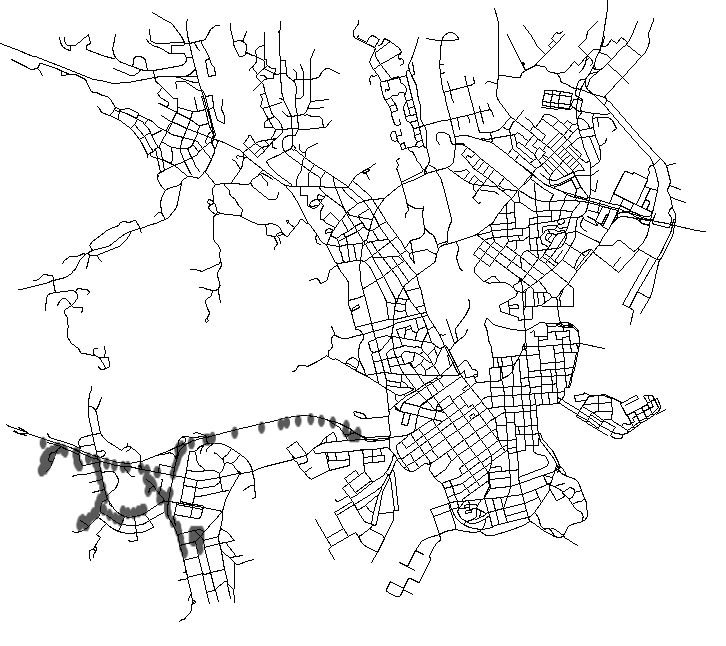
\includegraphics[scale=0.25]{../figure/mappa_0_hop.png}
    \caption{Explored area without use of delegations}
\end{figure}
\end{center}
\end{frame}

\begin{frame}
\frametitle{Risultati}
\begin{center}
\begin{figure}[ht]
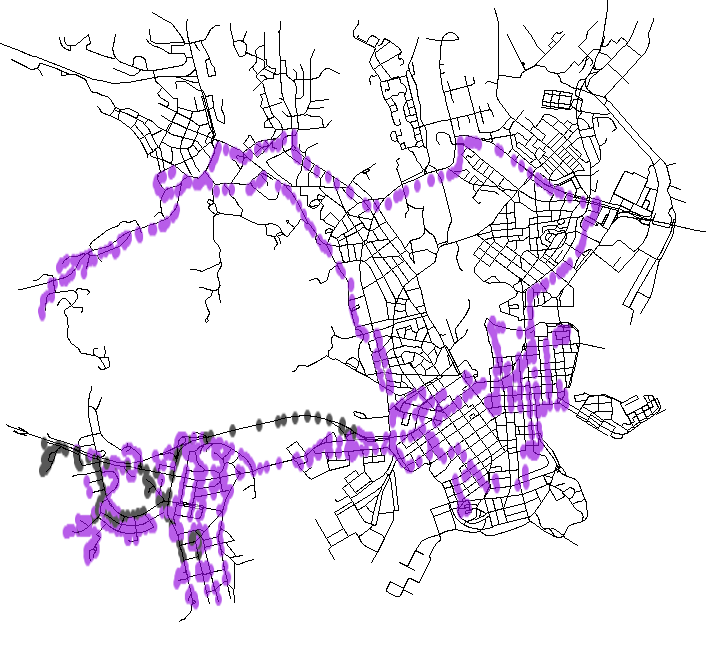
\includegraphics[scale=0.25]{../figure/mappa_1_hop.png}
    \caption{Explored area using M2MShare and 1-hop delegations}
\end{figure}
\end{center}
\end{frame}

\begin{frame}
\frametitle{Risultati}
\begin{center}
\begin{figure}[ht]
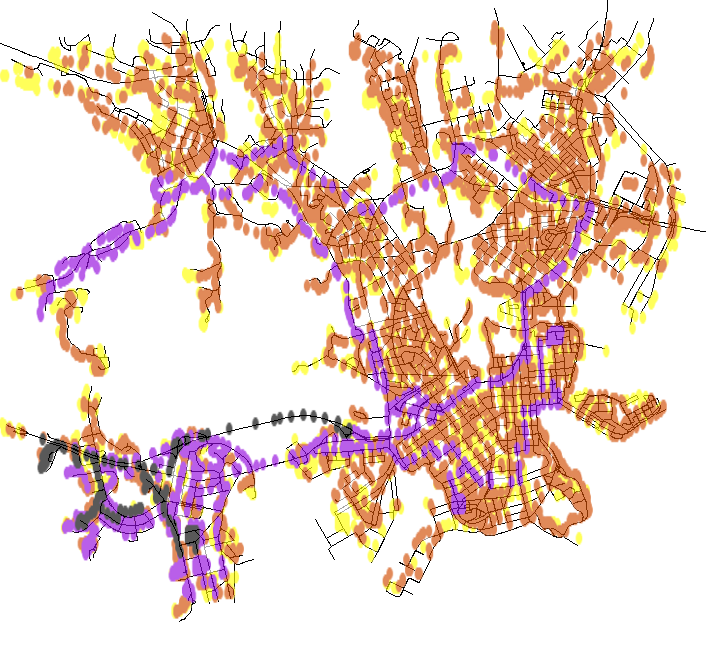
\includegraphics[scale=0.25]{../figure/mappa_3_hop.png}
    \caption{Explored area using M2MShare and up to 3-hop delegations}
\end{figure}
\end{center}
\end{frame}

\begin{frame}
\frametitle{Risultati}
\begin{center}
\begin{figure}[ht]
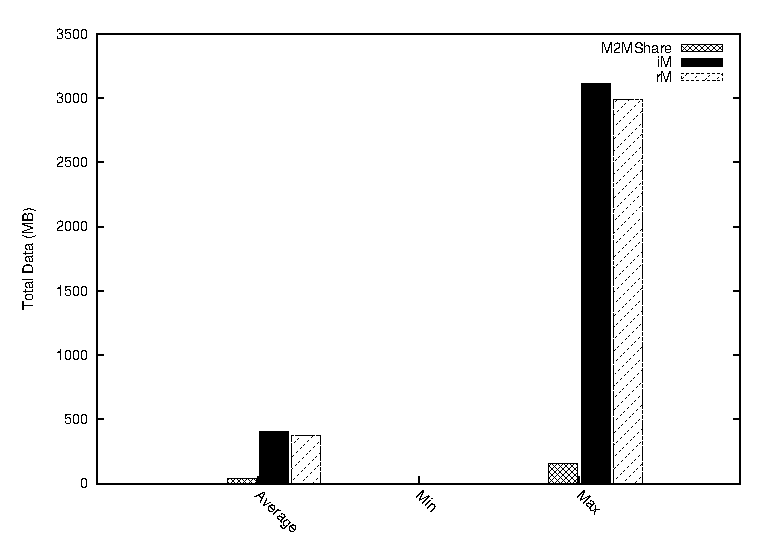
\includegraphics[scale=0.7]{../grafici/dataDFS_3MB.eps}
\caption{Average, min, max transferred data amount using different file division strategies and 3.0 MB file size.}
\end{figure}
\end{center}
\end{frame}

\begin{frame}
\frametitle{Risultati}
\begin{center}
\begin{figure}[ht]
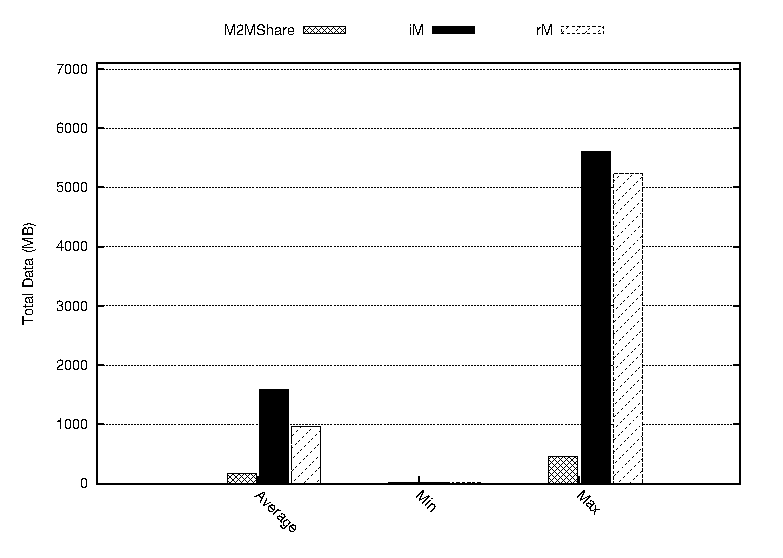
\includegraphics[scale=0.7]{../grafici/dataDFS_10MB.eps}
\caption{Average, min, max transferred data amount using different file division strategies and 10.0 MB file size.}
\end{figure}
\end{center}
\end{frame}

\begin{frame}
\frametitle{Risultati}
\begin{center}
\begin{figure}[ht]
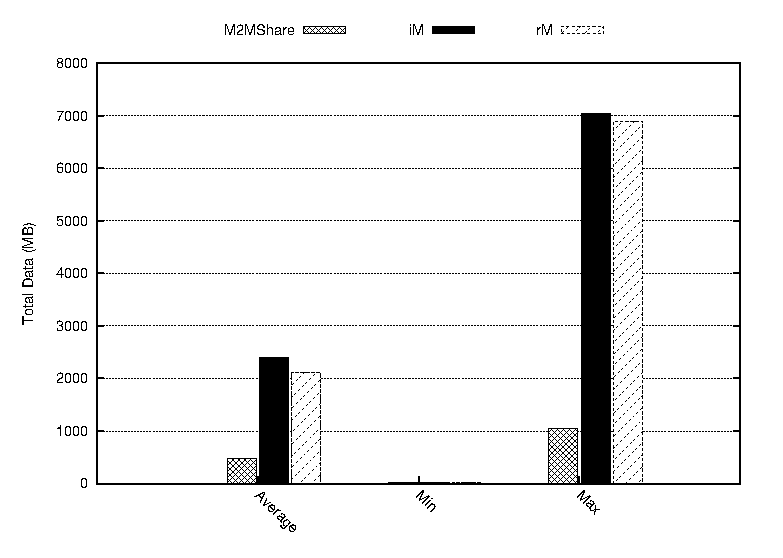
\includegraphics[scale=0.7]{../grafici/dataDFS_25MB.eps}
\caption{Average, min, max transferred data amount using different file division strategies and 25.0 MB file size.}
\end{figure}
\end{center}
\end{frame}

\begin{frame}
\frametitle{Riassumendo}

\begin{itemize}
\item Implementato M2MShare in un ambiente di simulazione realistico, che ci ha permesso di valutarne l'efficienza considerando la mobilità dei nodi interessati
\pause
\item Verificato l'efficienza di M2MShare rispetto altre strategie applicabili nello stesso contesto
\pause
\item Migliorare il protocollo esistente aggiungendo la possibilità di delega a più hops
\pause
\item Migliorato il simulatore ONE aggiungendo delle features condivise con la comunità di utenti
\pause
\item Alcuni risultati pubblicati durante Wireless Days Conference 2011 (\href{http://www.wireless-days.org/}{http://www.wireless-days.org}) in Niagara Falls, Ontario, Canada.
\end{itemize}
\end{frame}

\begin{frame}
\frametitle{\ }
\begin{center}
Grazie per l'attenzione.
\end{center}
\end{frame}



\end{document}